% MLSys 2027 submission (same format as MLSys 2025). Build: make
% Anonymous by default: do NOT add [accepted] until camera-ready.
\documentclass{article}

\usepackage{microtype}
\usepackage{graphicx}
\usepackage{subfigure}
\usepackage{booktabs}
\usepackage{amsmath}
\usepackage{xcolor}
\usepackage{hyperref}
\newcommand{\theHalgorithm}{\arabic{algorithm}}
\usepackage{mlsys2025}

% Drafting markers (see the Paragraph skeleton tab). Remove all before submission:
%   grep -n 'TODO\|SLOT\|\[\[FIG\|\[\[DIAG' paper/*.tex paper/sections/*.tex
\newcommand{\TODO}[1]{\textcolor{red}{[TODO: #1]}}
\newcommand{\SLOT}[1]{\textcolor{blue}{[SLOT: #1]}}

\mlsystitlerunning{What Do Static Computational Graphs Know About Hardware Performance?}

\begin{document}

\twocolumn[
\mlsystitle{What Do Static Computational Graphs Know About Hardware Performance?\\
An Information-Content Study of Learned TPU Layout Cost Models}

% Real names/affiliations go in only at camera-ready; the style prints
% "Anonymous Authors" in submission mode, and nothing identifying may be in the source.
\begin{mlsysauthorlist}
\mlsysauthor{Anonymous Author}{anon}
\end{mlsysauthorlist}
\mlsysaffiliation{anon}{Anonymous Institution}
\mlsyscorrespondingauthor{Anonymous Author}{anon@example.com}

\mlsyskeywords{learned cost models, TPU, XLA, graph neural networks, evaluation methodology}

\vskip 0.3in

\begin{abstract}
Learned cost models rank compiler configurations, but it is unclear how much of a configuration's
speed can be determined from the static graph alone. We approach this problem via TPUGraphs XLA
layout collections, using parameter-matched GNNs, five paired seeds and paired significance tests.
Our two apparent gains shrank below what our design can detect once we tuned the flat baseline's
learning rate. Hierarchy plus hardware-contention edges raise Kendall's $\tau$ on xla:default by
$+0.165$ ($p < .001$) at a shared learning rate, but by only $+0.002$ ($p = .88$) with both arms
tuned. A per-node MXU-utilisation feature cuts convolution Top-1 slowdown by 0.30 at the shared
rate, but by only 0.03 ($p = .17$) against a tuned baseline. With no models used, measured runtimes
show that convolution graphs are $2.8\times$ more layout-sensitive than other graphs, yet static
graph-level features do not predict this sensitivity. We conducted an audit of 20 papers that make
comparative claims about learned cost models and found that none runs a significance test on its
headline claim. Our own $+0.165$ result shows that passing seed, parameter-matching and significance
checks is not enough without a tuned baseline. We release the protocol and a power-analysis tool.
\end{abstract}
]

\printAffiliationsAndNotice{}

\section{Introduction}
\label{sec:intro}

XLA, the compiler behind Google's TPUs, must decide how to arrange each neural network's tensors in
memory. There are many valid arrangements, called layout configurations, and they run at measurably
different speeds on real hardware. Timing every candidate is slow and the search space is too large to
try exhaustively, so a learned cost model ranks the candidates from the program's graph instead of
keeping the compiler in the loop~\cite{phothilimthana2023tpugraphs,kaufman2021learned}. Layout matters
for a physical reason: the TPU's matrix multiply unit (MXU) works on fixed-size tiles, so the way data
is laid out changes how efficiently the MXU is used~\cite{jouppi2020domainspecific}.

Progress on these models is reported almost entirely as architecture comparisons: model X ranks
configurations better than model Y. GNNs over computation graphs have become the dominant
approach~\cite{phothilimthana2023tpugraphs,kaufman2021learned,deng2024polynormer}. Such comparisons
cannot show whether a gain is real unless they control for seed noise, model capacity and baseline
strength. In an audit of 20 papers that make these comparisons, none runs a significance test on its
headline claim, and 17 of 20 fail at least three of five rigor axes (Section~\ref{sec:audit}).

We therefore ask a different question: how much of a configuration's speed is knowable from the static
graph the predictor sees, and how much lives only in the compiler's dynamic tiling search? We answer it
at three levels:
\begin{enumerate}
\item Does the static graph carry the performance information, and does that depend on the workload?
\item Where, physically, does it fall short?
\item Can current evaluation practice detect effects of this size?
\end{enumerate}

At each level the answer turns on baseline strength. First, our tested alterations (hierarchy and
contention edges) to graph structure provided no detectable gain over a flat matched model in any of
the 4 collections once the baseline is tuned: on xla:default, an apparent $+0.165$ $\tau$ at a
shared learning rate falls to $+0.002$ ($p = .88$). Second, convolution graphs are $2.8\times$ more
layout-sensitive than other graphs in measured runtimes, but a per-node MXU feature that narrows
convolution slowdown from 1.42 to 1.12 at the shared rate leaves a gain below detection ($-0.03$, $p
= .17$) against a tuned baseline. Third, a result that can pass seed, parameter-matching and
significance checks can still be a baseline artefact, as our own $+0.165$ was. All results are on
TPUGraphs' validation graphs with runtimes Google measured; we ran no TPU.

Our contributions are:
\begin{itemize}
\item A controlled and power-analysed protocol for comparing learned cost models, applied to all four
  TPUGraphs layout collections.
\item A model-free measurement that localises the information gap to convolution on the MXU.
\item A pre-registered test of whether per-node MXU geometry closes that gap, with a scramble control, a
  tuned-baseline check and an oracle ceiling.
\item An audit of evaluation practice across papers in the field along with concrete recommendations
  (Section~\ref{sec:recs}), the released protocol and the power-analysis tool.
\end{itemize}

\section{Background}
\label{sec:background}

\subsection{The layout problem}
\label{sec:layout-problem}
A layout is the order of a tensor's dimensions in memory, for example \{1,0,2\} rather than \{0,1,2\}.
In TPUGraphs, XLA chooses layouts only at configurable nodes (convolution, dot and reshape), whose TPU
implementations are the most constrained, and derives every other node's layout from those
choices~\cite{phothilimthana2023tpugraphs}. A layout configuration is one set of choices across all
configurable nodes of a graph. The choices interact: when two connected operations use different
layouts, the compiler inserts a copy (a transpose) between them, so nodes cannot be optimised
independently and a whole-graph model is needed. XLA's autotuner finds 10--20\% speedups on production
models, but every candidate must be compiled and timed. A learned cost model therefore ranks the
candidates from the graph so that only the top few are timed~\cite{kaufman2021learned}. The graph is
the HLO input to XLA's layout-assignment step: nodes are tensor operations and edges are data flow.

\subsection{The four collections}
\label{sec:collections}
TPUGraphs' layout data come in four collections: two graph sources crossed with two sampling schemes.
The xla graphs come from the XLA regression benchmark and MLPerf, covering vision, NLP, speech and
recommendation; the nlp graphs are BERT variants that differ in layers, attention heads and hidden
size. Random sampling draws diverse candidates with widely spread runtimes, while default sampling runs
a genetic search from the compiler's default layout and yields similar candidates. Default is harder
than random~\cite{phothilimthana2023tpugraphs}, and we find xla harder than nlp
(Section~\ref{sec:result1}). Google measured every runtime on one TPU v3 core. The xla collections have
7 validation graphs each and the nlp collections 20; the released test files carry no runtimes, so
every number in this paper is on validation graphs.

\subsection{Related work}
\label{sec:related}
Learned cost models span tensor-program models (AutoTVM~\cite{chen2018learning},
TenSet~\cite{zheng2021tenset}, TLP~\cite{zhai2022deep}), basic-block throughput models
(Ithemal~\cite{mendis2019ithemal}, GRANITE~\cite{sykora2022granite}, with the analytical
Facile~\cite{abel2023facile} as counterpoint), whole-graph models on TPU and XLA (Kaufman et
al.~\cite{kaufman2021learned}, TPUGraphs~\cite{phothilimthana2023tpugraphs},
TGraph~\cite{khizbullin2024graph}, Polynormer~\cite{deng2024polynormer},
PerfSAGE~\cite{chai2023perfsage}) and program representations (ProGraML~\cite{cummins2021programl}).
Recent directions include NeuSight~\cite{lee2024forecasting}, compiler world
models~\cite{pan2026toward}, regression language models~\cite{akhauri2025regression} and
Omniwise~\cite{wang2025omniwise}. These works report progress as one model beating another. We do not
propose a new model; we test how much any static-graph model can know, and Section~\ref{sec:audit}
audits how such comparisons are tested.

\section{Why Layout Matters on the TPU}
\label{sec:hardware}

\subsection{The matrix unit}
\label{sec:mxu}
A TPU v3 chip has two cores, each with two MXUs; TPUGraphs timed one core, so each graph ran on two
MXUs~\cite{jouppi2020domainspecific}. Each MXU is a weight-stationary $128\times128$ grid of
multipliers that multiplies in bf16 and accumulates in fp32: a $128\times128$ block of weights sits in
the array while inputs stream through, with rows holding the reduction dimension $K$ and columns the
output channels $N$. A convolution maps to a matrix multiply with $M =$ batch $\times$ output
positions, $K = C_{\mathrm{in}} \times$ kernel height $\times$ kernel width and $N = C_{\mathrm{out}}$.
Each dimension is cut into 128-wide pieces and the last piece is zero-padded, so the useful fraction
along a dimension of size $d$ is $d / (\lceil d/128 \rceil \times 128)$ (Figure~\ref{fig:mxu}).
Section~\ref{sec:capstone} computes this utilisation for each convolution node.

\begin{figure}[t]
\centering
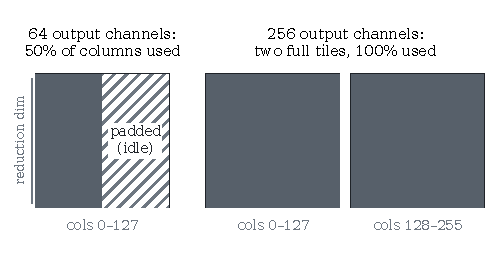
\includegraphics[width=\columnwidth]{figures/diag1_mxu_tiling.pdf}
\caption{A convolution's output channels map to the MXU's 128 columns. With 64 output channels, half
the columns sit idle as padding (left); 256 channels fill two tiles completely (right).}
\label{fig:mxu}
\end{figure}

\subsection{Tiling, roofline and contention}
\label{sec:tiling}
The compiler, not the graph, decides how each convolution is tiled onto the MXU: which dimensions to
tile and in what order, channel blocking, padding, and im2col versus direct convolution. Layout is an
input to these choices, because whether channels sit together in memory affects how they can be fed
into the array, so a layout change can change the tiling. The graph records operation types, shapes,
window sizes and layouts, but not the tiling the compiler chose. Part of a convolution's runtime
therefore depends on something no model sees (Section~\ref{sec:result2}), while the shape-based MXU
fit can still be computed from the graph (Section~\ref{sec:capstone}).

Whether MXU fit matters depends on the roofline. An operation whose arithmetic intensity (FLOPs per
byte moved) exceeds the ridge point, about 137 FLOPs/byte on TPU v3 (123 TFLOP/s $\div$ 900 GB/s), is
compute-bound, and its speed depends on how well it fills the MXU; below the ridge, memory bandwidth
dominates. Operations that need the same resource also compete for it: convolutions and dot products
share the core's two MXUs, and memory-moving operations (copy, transpose, reshape) share HBM bandwidth.
Our contention-edge model encodes this competition explicitly (Section~\ref{sec:models}).
\TODO{C11: the TPU v3 ridge $\approx$137 FLOP/byte is AI-verified only (VERIFICATION.md C11);
human-check the vendor source before submission}

\section{The Instrument: Method and Experimental Setup}
\label{sec:instrument}

\subsection{Task, inputs and metrics}
\label{sec:task}
Each model ranks a graph's layout configurations by runtime, using TPUGraphs' official train/validation
split for each collection. Models train with the ListMLE ranking loss~\cite{xia2008listwise} on up to
128 sampled configurations per graph per epoch; validation scores every configuration. Every model
receives the same static inputs: 140 features per node plus 18 layout features per configurable node.
These already include the convolution sizes (\texttt{shape\_dimensions} and \texttt{window\_size}) and
the kernel layout (layout features 12--17); we took the feature names from Google's featurizer source
and checked them against the data. The models therefore lack only the compiler's tiling and an
explicit MXU-utilisation number. We report Kendall's $\tau$, computed per graph and averaged across
graphs~\cite{kendall1938measure}, and Top-$K$ slowdown, the autotuner-facing metric: the best true
runtime among the model's top $K$ configurations divided by the best runtime overall.

\subsection{The three models}
\label{sec:models}
Each model adds one layer of structure while the parameter count stays roughly constant. The flat
baseline is GraphSAGE~\cite{hamilton2017inductive}: three SAGEConv layers with residual connections,
read out as a mean over all nodes plus a separate mean over configurable nodes, with hidden width 172
(236,157 parameters). The hierarchical model replaces flat message passing with two DiffPool pooling
stages~\cite{ying2018hierarchical}, the first clustering to at most 128 clusters (235,553 parameters).
The contention-edge model adds edge-aware GINE convolutions over the data-flow
edges~\cite{hu2019strategies} plus two edge types that link nearby operations competing for the matrix
unit (window of 5) and for memory bandwidth (window of 15) (234,120 parameters). These models are the
instruments being compared, not contributions.

\subsection{The protocol}
\label{sec:protocol}
Every comparison uses parameter-matched arms (within 0.3\% for flat and hierarchical, 0.9\% for
contention-edge), the same five seeds for every arm, and paired two-sided $t$-tests on
per-graph-averaged $\tau$ over held-out graphs, with Wilcoxon signed-rank tests as a direction check
and Benjamini--Hochberg correction across the three-arm family~\cite{benjamini1995controlling}. Each
control has a job. Seed-to-seed spread in $\tau$, about 0.04 to 0.07, is as large as the effects being
measured, so arms are paired by seed to cancel shared noise. Capacity differences fake wins: our
original ``DiffPool beats flat'' result came from 73\% more parameters (235,553 vs 136,321) and
vanished once the flat baseline was matched (Section~\ref{sec:xla-random}).

\subsection{Resolution of the design}
\label{sec:resolution}
With five seeds, the smallest detectable change in $\tau$ is 0.066--0.116 (Table~\ref{tab:mde}).
Effects below that are invisible to this design, not necessarily absent, and every null in this paper
is read against its minimum detectable effect (MDE). Detecting a change of 0.05 at a worst-case
$\sigma$ of 0.070 would need 18 seeds; because resolution improves only with the square root of the
seed count, the seed budgets common in this literature cannot resolve differences of the size papers
claim. The number of evaluation graphs matters less for the average: on xla:default, the bootstrap
standard deviation of $\tau$ is already stable at 7 graphs (median 0.0145, against 0.0131 at 20;
Appendix~C). It matters more for the 3-graph convolution subset in Section~\ref{sec:capstone}, which
we test with leave-one-graph-out and held-out-family checks.

\begin{table}[t]
\caption{Minimum detectable change in Kendall's $\tau$ (paired $t$-test, $\alpha = 0.05$, power 0.8)
by number of seeds $n$ and seed-to-seed standard deviation $\sigma$ of $\Delta\tau$.}
\label{tab:mde}
\centering
\small
\setlength{\tabcolsep}{4pt}
% Generated by scripts/paper_figures.py via power_analysis.min_detectable_effect
% (paired t, alpha=0.05, power=0.8)
\begin{tabular}{lcccccc}
\toprule
$\sigma$ (paired) & $n=3$ & $n=5$ & $n=7$ & $n=10$ & $n=15$ & $n=20$ \\
\midrule
0.040 & 0.124 & 0.066 & 0.051 & 0.040 & 0.031 & 0.026 \\
0.055 & 0.170 & 0.091 & 0.070 & 0.055 & 0.043 & 0.036 \\
0.070 & 0.217 & 0.116 & 0.089 & 0.070 & 0.054 & 0.046 \\
\bottomrule
\end{tabular}

\end{table}

\subsection{Evaluation choices}
\label{sec:eval-choices}
Two choices shape the numbers. First, all models use BatchNorm with batch statistics, so a
configuration's score depends on the evaluation batch it is scored in. $\tau$ comparisons use
evaluation batch 8; the Top-1 analyses in Sections~\ref{sec:result2} and~\ref{sec:capstone} use batch
32, their registered batch. Appendix~C gives every headline contrast at both, and the text notes each
case where the batch changes a verdict. Second, all arms train at one shared learning rate of 1e-3,
which matches them but does not tune them; Sections~\ref{sec:result1} and~\ref{sec:capstone} report the
pre-registered checks that tune each arm. The exception is nlp:default, whose amended runs use 1e-4 for
both arms (Section~\ref{sec:nlp-default}).

\section{Result I: Added Structure Gives No Detectable Gain over a Matched Flat Model}
\label{sec:result1}
In all four collections, no structured model beats the matched flat model. The scope differs by
collection: on xla:default both arms are learning-rate tuned; on nlp:default both run at a matched 1e-4
(exploratory); on xla:random and nlp:random all arms share 1e-3; and the hierarchical model was tested
only on the xla collections. The one result that looked like a clear win, on xla:default, did not
survive the pre-registered baseline check.

\subsection{xla:random: no gain from hierarchy or contention edges}
\label{sec:xla-random}
The hierarchical model does not beat the parameter-matched flat model: $\tau = 0.2645 \pm 0.0230$
against $0.2880 \pm 0.0365$, $\Delta\tau = -0.0235 \pm 0.0214$ ($p = .07$), with a point estimate that
leans negative. The contention-edge model scores $0.2640 \pm 0.0360$, $\Delta\tau = -0.0241 \pm
0.0665$ ($p = .46$); its large seed spread puts the MDE near 0.11. Top-$K$ slowdown is also null at
every $K$ (all $p \geq .45$), so neither model improves the configurations an autotuner would actually
try. On the convolution graphs' Top-1, the metric of Section~\ref{sec:capstone}, neither model differs
from flat either (hierarchical $+0.022$, $p = .77$; contention-edge $+0.003$, $p = .97$; MDE about
0.27). We checked the edge construction against a dense reference implementation, which agreed to
within 1e-7. Checkpoints were chosen at evaluation batch 32 but scored at batch 8; 12 of the 15 chosen
checkpoints are from the final epoch, and the conclusions hold at both batches.

\subsection{nlp:random: contention edges are marginally worse}
\label{sec:nlp-random}
On nlp:random's 20 validation graphs, the contention-edge model is marginally worse than flat:
$\tau = 0.6408 \pm 0.0334$ against $0.7129 \pm 0.0577$, $\Delta\tau = -0.0722 \pm 0.0583$
($p = .0504$). Top-$K$ agrees at $K = 5$ and 10 and is not significant at $K = 1$ or 100. Both arms
share lr 1e-3 and this model is learning-rate sensitive, so an under-tuned contention-edge model is a
possible explanation.

\subsection{xla:default: an apparent large win at the shared learning rate}
\label{sec:xla-default}
At the shared lr of 1e-3, both connectivity models appear to beat the flat model by a wide margin
(Figure~\ref{fig:staircase}). The flat baseline scores $\tau = 0.0327 \pm 0.0135$, the hierarchical
model $0.1484 \pm 0.0276$ and the contention-edge model $0.1977 \pm 0.0133$, so contention-edge $-$
flat is $\Delta\tau = +0.1650 \pm 0.0133$ ($p < .001$). The contention-edge model wins on all five
seeds, the margin is about 12 times the seed spread, the arms are parameter-matched, and the result
survives Benjamini--Hochberg correction. It passes audit Axes 1--3 and most papers would report it as
a win. One graph carries much of it (inception\_v3, $\Delta\tau$ $+0.550$; the other six average
$+0.101$), and Appendix~A decomposes the gain into hierarchy and edge components. The warning sign is
the flat model itself: $\tau = 0.033$ is barely better than random ranking ($\tau = 0$).

\begin{figure}[t]
\centering
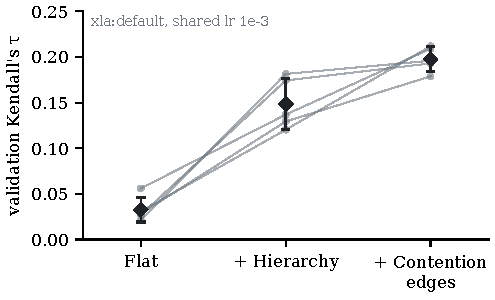
\includegraphics[width=\columnwidth]{figures/fig_r1_xla_default_staircase.pdf}
\caption{At a shared learning rate of 1e-3, adding hierarchy and then contention edges appears to raise
validation Kendall's $\tau$ on xla:default from 0.033 to 0.198. Grey lines join the five paired seeds;
black markers show mean $\pm$ std (evaluation batch 8). Section~\ref{sec:tuning} shows that the rise
comes from an untuned flat baseline.}
\label{fig:staircase}
\end{figure}

\subsection{Tuning the baseline dissolves the win}
\label{sec:tuning}
We trained each model at five learning rates (3e-5, 1e-4, 3e-4, 1e-3 and 3e-3) and kept each model's
best by validation $\tau$ (Figure~\ref{fig:lr}). The flat model is best at 1e-4 and collapses at 1e-3,
the shared rate. Against the tuned flat baseline, the contention-edge model at 1e-3 is no longer a win
(though not significantly worse), and the hierarchical model is worse. With both arms tuned, the
contention-edge model is also best at 1e-4 and no difference is detected: $\Delta\tau = +0.002$
($p = .88$, MDE 0.037). Tuning raised the flat model by $+0.193$ $\tau$ but the contention-edge model by
only $+0.029$, so the original $+0.165$ was mostly the flat model being held back. The best rates were
picked on the same validation set that is scored, within a 50-epoch budget in which most runs peaked at
epoch 46 or later; both limitations apply equally to both arms.

We call this the baseline-strength pattern: a gain measured against an untuned baseline that shrinks
below detection once the baseline is tuned. It recurs twice in Section~\ref{sec:capstone}.

\begin{figure}[t]
\centering
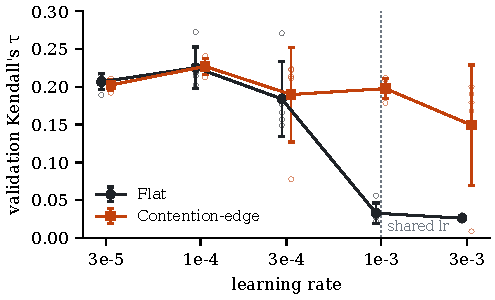
\includegraphics[width=\columnwidth]{figures/fig_r4_lr_curves.pdf}
\caption{Validation $\tau$ on xla:default at five learning rates for the flat and contention-edge
models (open circles: seeds; filled: mean $\pm$ std; 50-epoch budget). The flat model's collapse at the
shared rate of 1e-3 (dashed line) produces the apparent gain in Figure~\ref{fig:staircase}; at each
model's best rate the two are indistinguishable.}
\label{fig:lr}
\end{figure}

\subsection{nlp:default: a training failure, then an amended run}
\label{sec:nlp-default}
At the shared lr of 1e-3, the contention-edge model did not train on nlp:default: from the first epoch
it gave every layout the same score (seeds 42 and 100), so $\tau$ is undefined on all 20 validation
graphs. We recorded this as a training failure before reading the relevant results (Amendment~1,
Appendix~B); it says nothing about the information the graph carries. An exploratory rerun of both arms
at 1e-4, a rate chosen after seeing the failure, finds no difference: $\tau = 0.4087$ against flat's
$0.4138$, $\Delta\tau = -0.0051$ ($p = .53$, MDE 0.027). Compared with flat at the untuned 1e-3, the
contention-edge model would have looked like a winner ($+0.089$, $p = .02$), but flat itself gains
$+0.095$ from the lower rate. Across collections, the apparent advantages come from the learning rate,
not the connectivity. We next ask where the remaining error lies.

\section{Result II: The Information Gap Is in Convolution on the MXU}
\label{sec:result2}

\subsection{The remaining error is concentrated on convolution graphs}
\label{sec:conv-error}
Ranking errors pile up on convolution graphs (Figure~\ref{fig:conv}). On xla:random's 7 validation
graphs, averaging the flat and contention-edge models over five seeds at the shared lr, the top-ranked
layout is 1.44--1.51$\times$ slower than the best on the three convolution-dominated graphs, against
1.01--1.07$\times$ on the other four (UNet-3D and three BERT variants, which are memory- or
matmul-bound). At evaluation batch 8 the ranges are 1.21--1.52$\times$ and 1.01--1.08$\times$, so every
convolution graph is still worse than every other graph. The grouping was chosen after seeing the
results, so it is exploratory; the rest of this section tests it without models.

\begin{figure}[t]
\centering
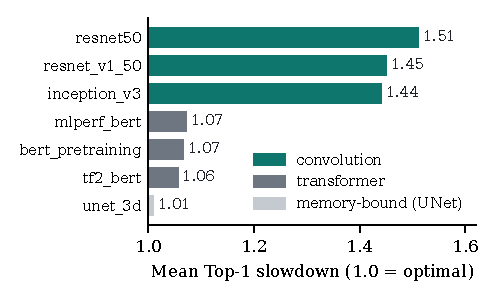
\includegraphics[width=\columnwidth]{figures/fig_c1_conv_failure.pdf}
\caption{Per-graph Top-1 slowdown on xla:random's validation graphs, averaged over the flat and
contention-edge models and five seeds (shared lr 1e-3, evaluation batch 32; 1.0 = optimal). The three
convolution graphs are 44--51\% slower than the best layout; the others are 1--7\% slower.}
\label{fig:conv}
\end{figure}

\subsection{Measured runtimes alone show the gap}
\label{sec:model-free}
For each graph--collection pair we computed the spread of measured runtimes across layouts
(coefficient of variation). The median spread is 0.239 across 95 convolution-bearing pairs against
0.086 across 49 convolution-free pairs: convolution-bearing graphs vary 2.77 times as much
(Mann--Whitney $p = 1.5\times10^{-7}$). Across all 144 pairs, the share of a graph's compute that runs
on the MXU correlates with its runtime spread (Spearman $\rho = +0.52$). A model that ranks convolution
graphs poorly therefore faces a harder problem, not merely a failure of prediction.

\subsection{The physical reason}
\label{sec:physical}
In the 4 convolution-bearing validation graphs, every convolution has an arithmetic intensity between
90 and 2,900 FLOPs/byte, all above the TPU v3 ridge. Every convolution is therefore compute-bound, and
its runtime is set by how efficiently its tiling uses the MXU. A layout change can alter the tiling and
with it the padding waste and the speed, and that tiling is exactly what the graph does not record.
\TODO{FACT ERROR, fix in your words: erratum 9648419 (2026-10-13) says NOT every conv is above the
ridge. Per op, 11--26\% of conv ops are below 137 FLOP/byte (1--16\% of MACs); per-op intensity spans
3.8--11,810. Correct claim: conv work is predominantly compute-bound (74--89\% of ops, 84--99\% of MACs;
MAC-weighted intensity 688--2,857). Source: experiments/phase8_mxu_misalignment.md, Erratum.}

\subsection{Three simple static explanations fail}
\label{sec:static-fail}
% REVISE-IF-TIME: low 4-gram overlap with the First Draft.
If the sensitivity could be read off simple static summaries, a model should not need the compiler's
tiling. Three such summaries fail. (a)~Channel-padding waste does not predict runtime spread across
convolution graphs ($\rho = -0.06$, $n = 95$, $p = .53$): no detectable correlation. (b)~Roofline
position does not order failure: UNet-3D, the most MXU-intense graph (intensity $\approx$ 2,857), is
handled best at 1.01$\times$, while the failing graphs sit near 690--730 (Inception 1.44$\times$,
ResNet-v1-50 1.45$\times$, ResNet-50 1.51$\times$). (c)~Within-convolution MXU overhead runs opposite
to slowdown: Inception has the highest overhead (1.69) and the lowest slowdown of the three, the
ResNets the lowest (1.17) and the highest. Checks (b) and (c) are illustrations on 4 and 3 graphs, not
tests.

This does not contradict Section~\ref{sec:capstone}. Here we ask a between-graph question: does a
graph's average padding waste predict its runtime spread? Section~\ref{sec:capstone} asks a
within-graph one: does per-node MXU geometry, given to the model, help rank configurations inside a
graph? Our explanation for the gap, that the graph omits the compiler's tiling choice, is inferred from
these results; we did not observe that choice directly.

\section{Capstone: What a Per-Node MXU Feature Recovers}
\label{sec:capstone}

\subsection{A large gain at the shared learning rate}
\label{sec:capstone-shared}
% REVISE-IF-TIME: low 4-gram overlap with the First Draft.
We added one number to each convolution node, its channel-padding utilisation
(Section~\ref{sec:mxu}), and kept everything else identical to the flat baseline. The test set is
pre-registered: three convolution graphs (inception\_v3, resnet50.4x4.fp16, resnet\_v1\_50) on
xla:random and xla:default, with the four BERT and UNet graphs as a placebo. At lr 1e-3, convolution
Top-1 slowdown drops from 1.42 to 1.12, $\Delta = -0.30$ (Benjamini--Hochberg $p = .0032$, Cohen's
$d = -3.15$; Table~\ref{tab:arms}). The channel arm wins on all 6 graph--collection instances and on
all five seeds (Wilcoxon $p = .062$, the floor for five seeds), while the placebo graphs barely move
(1.0272 to 1.0292). The scramble control rules out extra capacity: shuffling the feature's values
between nodes keeps the input width but removes the information, and the real feature beats it
($\Delta = -0.244$, $p = .006$; rerun on matched GPU hardware, $-0.221$, $p = .003$). Spatial-only and
combined encodings also help, though the combined arm nudges the placebo graphs too. Before running
anything, we had predicted that the channel-only arm would not help; it was the strongest.

\begin{table*}[t]
\caption{Convolution (CONV, 3 graphs) and placebo (OTHER, 4 graphs) Top-1 slowdown for each MXU
encoding against the untuned baseline at the shared lr of 1e-3 (mean $\pm$ std over 5 paired seeds;
evaluation batch 32; verdicts unchanged at batch 8). BH-$p$ is Benjamini--Hochberg-adjusted over the
three arms.}
\label{tab:arms}
\centering
\small
% Generated by scripts/paper_figures.py from experiments/phase8c_results.json
\begin{tabular}{lccccc}
\toprule
Arm & CONV slowdown & OTHER slowdown & $\Delta$ CONV & BH-$p$ & $d$ \\
\midrule
baseline & 1.4246 $\pm$ 0.0721 & 1.0272 $\pm$ 0.0027 & -- & -- & -- \\
channel & 1.1203 $\pm$ 0.1077 & 1.0292 $\pm$ 0.0182 & -0.3043 & 0.0032 & -3.15 \\
spatial & 1.1758 $\pm$ 0.0389 & 1.0237 $\pm$ 0.0080 & -0.2488 & 0.0014 & -4.72 \\
full & 1.1933 $\pm$ 0.1479 & 1.0125 $\pm$ 0.0080 & -0.2313 & 0.0073 & -2.25 \\
\bottomrule
\end{tabular}

\end{table*}

\subsection{Against a tuned baseline, the gain is below detection}
\label{sec:capstone-tuned}
% REVISE-IF-TIME: low 4-gram overlap with the First Draft.
The baseline above is Section~\ref{sec:result1}'s handicapped arm: the same flat model at lr 1e-3,
which learns (overall $\tau = 0.2311$) but is undertrained, with 4 of 5 runs peaking at the final
epoch. A pre-registered check reran both arms over a grid of learning rates and kept each arm's best;
both landed on 3e-5, the lowest rate in the grid, so tuning may not have fully converged. Tuning alone
takes the baseline from 1.42 to 1.09, removing most of the convolution error. The channel feature's
remaining gain is $\Delta = -0.033$ ($p = .17$), below the five-seed MDE of 0.073. The tuned baseline
left so little room that no five-seed outcome could have reached significance under the registered
test. At evaluation batch 8 the gain is nominally significant ($-0.060$, $p = .045$), but the placebo
graphs move too ($p = .044$), and the registered batch is 32. This is the second instance of the
baseline-strength pattern.

\subsection{Robustness and generalisation}
\label{sec:capstone-robust}
The shared-rate result rests on three graphs from two families (Inception and ResNet). Dropping any one
graph still leaves a clear effect ($\Delta$ $-0.26$ to $-0.38$, all $p \leq .0099$; post hoc). On 19
instances from 6 convolution families the model never trained on, with both arms tuned, the gain points
the right way but is not significant ($\Delta$ $-0.11$, $p = .35$, MDE 0.39), and its direction flips
at evaluation batch 8. This test cannot say whether the feature generalises. Figure~\ref{fig:forest}
summarises every arm.

\begin{figure}[t]
\centering
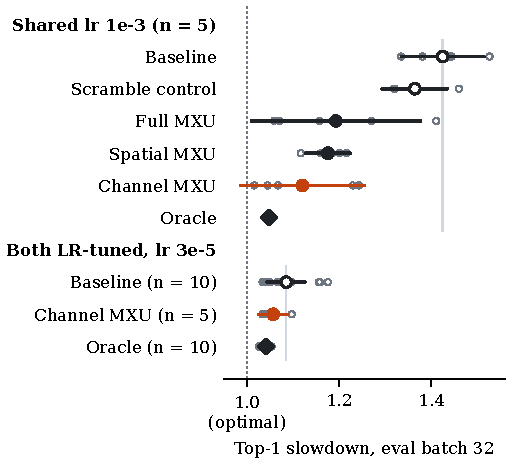
\includegraphics[width=\columnwidth]{figures/fig_k1_forest.pdf}
\caption{Convolution Top-1 slowdown per arm (mean, 95\% $t$-interval and seeds; evaluation batch 32;
1.0 = optimal). Top: at the shared lr of 1e-3, all three MXU encodings beat the baseline and the
scramble control. Bottom: with arms tuned at 3e-5, the baseline reaches 1.09 and neither the channel
feature nor the oracle is detectably better. The tuned baseline and oracle come from the 10-seed R5
run; the tuned channel arm comes from the 5-seed tuning check.}
\label{fig:forest}
\end{figure}

\subsection{The oracle ceiling}
\label{sec:oracle}
To bound how good a static model could get, we built an oracle that receives information derived from
the measured runtimes, so it cheats by design. At lr 1e-3 it reached 1.048, far ahead of the baseline,
with the channel arm in between. Our pre-registered prediction P5 required the oracle both to reach 1.05
and to beat the channel arm significantly; it reached the bar but not significance (gap 0.0725,
$p = .19$), so P5 is not confirmed. A power analysis done afterwards shows P5 could not have passed:
reaching 1.05 capped the oracle's possible advantage at 0.0703, below the five-seed MDE of
0.091--0.116, and the observed gap would have needed about 18 seeds. At evaluation batch 8 the gap is
significant ($-0.099$, $p = .020$), but the registered batch is 32. Our own pre-registration fell into
the under-powering trap that Section~\ref{sec:audit} describes.

We then re-ran the oracle against a tuned baseline, choosing 10 seeds by a power check before running.
At the registered batch 32, the oracle's lead is not detected ($\Delta$ $-0.043$, $p = .056$, MDE
0.062); at batch 8 it is significant in the same direction ($\Delta$ $-0.093$, $p = .003$). On the
placebo graphs the oracle does slightly worse than the baseline. Tuning barely moved the oracle but
moved the baseline a lot, so most of the headroom seen at 1e-3 came from the untuned baseline: the third
instance of the pattern. The lr-1e-3 oracle checkpoints all came from epoch 5 and were trained on CPU,
so the comparison between the two oracle runs is descriptive only.

\subsection{What remains open}
\label{sec:open}
Whether any convolution gap remains after tuning is unresolved at our seed count as the gap was
inconclusive (not detected) at batch 32 and only significant at batch 8. The registered reading of
this outcome is that label noise, which is the variation in measured runtimes from run-to-run, is
the deeper limit, but our test cannot separate label noise from information missing from the graph.
Answering the question would potentially need more seeds and more convolution graphs than three
graphs from two families.

\section{Result III: The Audit}
\label{sec:audit}
% Every percentage: "a purposive sample of 20", never "the field". No paper named as a failure.

\subsection{Method}
\label{sec:audit-method}
We scored a purposive sample of 20 papers (2018--2026) that make a comparative architectural claim
about a learned performance or cost model on five rigor axes: (1)~seed variance, (2)~parameter
matching, (3)~significance testing, (4)~evaluation-set integrity, and (5)~effect size against noise and
baseline strength. Each axis is scored pass, partial or fail, and every score is backed by a quoted
passage.

Papers were selected by snowball sampling from the lineage of learned cost model papers plus searches;
the search terms were not logged and the selection protocol was written afterwards. All 20 papers were
first scored by AI. Five were then human-verified on all five axes, which corrected 3 of 25 scores, all
towards stricter; Axis 3 was human-verified for all 20 because the pre-screen failed every paper on it.
The only score that became looser was TPUGraphs, from fail to partial, because it reports $\pm1\sigma$
but runs no test. For the other 15 papers, Axes 1, 2, 4 and 5 are AI-prescreened only. To estimate
coverage, 6 fixed Semantic Scholar queries returned 571 candidates; our sample includes 8 of the 30
most-cited in-scope papers and 0 of the 10 most-cited from 2024--2026. That screening retrieves only 10
of our 20 papers (it misses TPUGraphs), and in-scope papers outside the sample were not audited.

\subsection{No paper runs a significance test}
\label{sec:audit-result}
None of the 20 papers runs a significance test on its headline architectural claim, 17 (85\%) fail at
least three of the five axes, and none passes Axes 1--3 together (Table~\ref{tab:audit}).
% Frame B (O15): sentence fixed in advance by the frozen declaration (section 6, "0 of n"), counts 0/10.
In a separate, pre-declared check of the 10 most-cited in-scope papers from 2024--2026 in the same
frame, none of the 10 we could score runs a significance test for its headline comparison
(Appendix~D).

\begin{table}[t]
\caption{Audit outcome by rigor axis for 20 papers that make a comparative architectural claim about a
learned performance or cost model (2018--2026). No paper passes Axes 1--3 together, and 17 of 20 fail
at least three of the five axes.}
\label{tab:audit}
\centering
\small
% Generated by scripts/paper_figures.py from the per-paper tables in experiments/phase7_meta_analysis.md
% papers failing >=3 axes: 18/20; passing axes 1-3: 0/20
\begin{tabular}{lccc}
\toprule
Axis & Fail & Partial & Pass \\
\midrule
1. Seeds / variance & 16/20 & 4/20 & 0/20 \\
2. Parameter-matched & 17/20 & 3/20 & 0/20 \\
3. Significance test & 20/20 & 0/20 & 0/20 \\
4. Eval-set integrity & 4/20 & 7/20 & 9/20 \\
5. Effect vs noise & 6/20 & 14/20 & 0/20 \\
\bottomrule
\end{tabular}

\end{table}

\subsection{Typical practice cannot resolve effects of this size}
\label{sec:audit-resolve}
These failures are not missing paperwork. No paper reports the seed-to-seed spread of its headline
comparison, so readers cannot discern whether a gain exceeds the noise. By Table~\ref{tab:mde}, five seeds
resolve only $\Delta\tau \approx$ 0.07--0.12, and the effects in Sections~\ref{sec:result1}
and~\ref{sec:capstone} are smaller. Our own results show both failure modes. The DiffPool win only came from
capacity and vanished at matched size (Section~\ref{sec:protocol}). The $+0.165$ contention-edge result
had five seeds, matched parameters and $p < .001$, passing Axes 1--3, yet only the pre-registered
baseline check exposed it as a learning-rate handicap (Section~\ref{sec:tuning}). Passing every check
the field currently applies is not enough.

\subsection{Good practice already exists}
\label{sec:audit-good}
The problem is a habit, not a rule. Kaufman et al.\ report a case where their own learned model loses to
the analytical baseline on the harder split of their tile-size task (6.3\% against 2.3\% mean
error)~\cite{kaufman2021learned}. PerfVec declines a head-to-head state-of-the-art claim because the
hardware differed~\cite{li2024learning}. HLS-GNN runs a five-seed protocol~\cite{wu2022highlevel}. Rigorous comparison is achievable within current practice.

\section{Recommendations and Released Artifacts}
\label{sec:recs}
% Link = the ANONYMOUS repository only (never the live repo or wandb).
Based on our results, we propose six changes to practices for comparing learned cost models. The first three correspond to
audit Axes 1--3; the fourth catches what those three miss, as Section~\ref{sec:tuning} shows.
\begin{enumerate}
\item Report the seed-to-seed spread of the headline difference, and pair seeds across arms.
\item Match parameter counts across arms, or report results at several matched sizes.
\item Run a paired significance test on the headline comparison and report its effect size.
\item Tune the baseline with the same budget as the proposed model, and report both learning-rate
  curves.
\item Compute the minimum detectable effect before running, choose seeds and evaluation graphs so the
  claimed effect lies above it, and read every null against it.
\item Report evaluation choices that have the potential to change a verdict, such as the evaluation batch under
  batch-statistic normalisation.
\end{enumerate}

To support these practices, we release, in an anonymous repository for review
(\url{https://github.com/falconcloaknmardoll/static-graph-perf}), the following: the protocol, every
pre-registration with its amendments and commit history, the 140-feature map naming each node feature
(including those that carry convolution sizes), and \texttt{power\_analysis.py}. Given seed noise, the
tool returns the MDE for $n$ paired seeds, and when given a per-graph $\tau$, it estimates how fast the aggregate's
spread shrinks as evaluation graphs are added.

\section{Limitations and Conclusion}
\label{sec:conclusion}

\subsection{Limitations}
\label{sec:limitations}
\paragraph{Data and hardware.} We use one benchmark and its validation split. xla:default has 7
validation graphs and the Section~\ref{sec:capstone} convolution subset only 3. We ran no TPU, so
results describe ranking quality on TPUGraphs' measured runtimes, not end-to-end compiler speedups.

\paragraph{Statistics and tuning.} With five seeds, the MDE is 0.037--0.116 for the main contrasts and
up to 0.39 for small subsets, and two runs of the identical flat recipe differ by 0.057 $\tau$
($p = .08$), so a null means ``not detected above the MDE''. Learning rates were tuned for two contrasts
only, picked on the scored validation set, and in Section~\ref{sec:capstone} the best rate sat at the
grid edge; ``tuned'' means tuned within this recipe, and the other collections are compared at one
shared rate.

\paragraph{Baseline strength and measurement.} Our tuned flat model scores 1.2--2.1$\times$ the
TPUGraphs baseline on all four collections but below TGraph on all four (xla:default 0.23 against 0.48),
and below TGraph's no-edges ablation on both xla collections, under different protocols. Our findings
hold for a matched, mid-strength GNN; whether they hold at state-of-the-art strength is untested. Scores
depend on the evaluation batch, and the lr-1e-3 scramble and oracle arms trained on CPU while all others
trained on GPU; the text flags each verdict the batch changes. The audit covers a purposive sample in
which 5 papers were fully human-verified and all 20 on Axis 3, so it describes this sample, not the
whole field.

\subsection{Conclusion}
Static graphs carry less learnable advantage than the shared-learning-rate comparisons suggest: both
apparent gains shrank below detection once the baseline was tuned (connectivity $+0.165$ to $+0.002$
$\tau$; MXU feature $-0.30$ to $-0.03$ convolution Top-1). The hardware does impose a real limit on
convolution graphs, which are $2.8\times$ more layout-sensitive in measured runtimes, yet a tuned flat
model already brings their Top-1 slowdown from 1.42 to 1.09. A comparison can pass seed,
parameter-matching and significance checks and still be a baseline artefact, and none of the 20 audited
papers runs the significance test. The open question is not how to close a known gap but whether, after
tuning, any residual gap exists at all.


% No acknowledgments in the submission (anonymity). Add at camera-ready.

\bibliography{refs}
\bibliographystyle{mlsys2025}

\section*{AI Usage Disclosure}
\textit{Tools.} We used Claude Code with Anthropic's Claude models throughout the project.

\textit{Ideation and experiment design.} We discussed research questions, robustness checks and
pre-registrations with Claude, and it drafted parts of those documents.

\textit{Literature search and audit.} Claude screened the 571 coverage candidates and produced the
first-pass audit scores. Human verification is as stated in Section~\ref{sec:audit}.

\textit{Code.} Claude wrote most of the training, evaluation, statistics and figure code under the
first author's direction.

\textit{Data.} No data were generated by AI. All runtimes come from TPUGraphs.

\textit{Writing.} The first author wrote the complete first draft, which set out the paper's argument,
results and interpretation. Claude was then used for language editing, condensing the text to the page
limit and checking for inconsistencies. It also drafted some summary and recommendation text and the
appendix prose from the authors' results, which the authors reviewed and revised.

The authors take responsibility for all content.

\end{document}
